\pdfvariable minorversion 7\relax
\documentclass[aspectratio=169]{rosenpass-beamer}
\usepackage[english]{babel}
\usepackage{booktabs}

\usepackage{tikzsymbols}
\usepackage{multirow}
\usepackage{stmaryrd}
\usepackage[dvipsnames]{xcolor}

\newcommand*{\heading}[1]{%
  {
    \hspace*{-0.5cm}#1
    \vspace{1.0em}
  }
}

%TODO Short title for the headline?
\title{Sicherheit\textsuperscript{2}}
\subtitle{\texorpdfstring{\vspace{0.2em}}{}Das Zusammenspiel von Safety \& Security im Fokus der Kryptoagilität}
\author[Karolin Varner, Wanja Zaeske]{Karolin Varner \& Wanja Zaeske}
\institute{\url{https://rosenpass.eu}}

\conference{CAST-Workshop}
\date{2025-05-15}

\usepackage{biblatex}
\addbibresource{sources.bib}

\graphicspath{{}{graphics/}}

\usepackage{transparent}
\usepackage{colortbl}
\usepackage{pdfpc}

% Syntaxerweiterung \SetNextBackground{Bild} oder image= option bei frame

\partnerlogo{%
	\includegraphics[height=2\baselineskip]{MPI-SP}%
	\includegraphics[height=2\baselineskip]{dlr}%
}

\ExplSyntaxOn
\tl_gset:Nn \g__ptxcd_interlude_prefix_tl  {artsy-slide-backgrounds-smaller-hd/artsy-mild-bg-2}
\int_gset:Nn \g__ptxcd_interlude_page_int {-1}
\ExplSyntaxOff

\begin{document}

\maketitle

\newcommand*{\citePqwgUrl}{https://eprint.iacr.org/2020/379}
\newcommand*{\citePqwgCode}{PQWG}
\newcommand*{\citePqwg}{\href{\citePqwgUrl}{[\citePqwgCode]}}

\newcommand*{\citeGhpUrl}{https://eprint.iacr.org/2018/024}
\newcommand*{\citeGhpCode}{GHP}
\newcommand*{\citeGhp}{\href{\citeGhpUrl}{[\citeGhpCode]}}

\newcommand*{\citeHpkeUrl}{https://eprint.iacr.org/2020/1499}
\newcommand*{\citeHpkeCode}{HPKE}
\newcommand*{\citeHpke}{\href{\citeHpkeUrl}{[\citeHpkeCode]}}

\newcommand*{\citeXwingUrl}{https://eprint.iacr.org/2024/039}
\newcommand*{\citeXwingCode}{XWING}
\newcommand*{\citeXwing}{\href{\citeXwingUrl}{[\citeXwingCode]}}

\newcommand*{\citeNoiseUrl}{https://noiseprotocol.org/noise.html}
\newcommand*{\citeNoiseCode}{NOISE}
\newcommand*{\citeNoise}{\href{\citeNoiseUrl}{[\citeNoiseCode]}}

\newcommand*{\citeBellareRogawayUrl}{https://eprint.iacr.org/2004/331}
\newcommand*{\citeBellareRogawayCode}{BR06}
\newcommand*{\citeBellareRogaway}{\href{\citeBellareRogawayUrl}{[\citeBellareRogawayCode]}}

\newcommand*{\citeHaleviUrl}{https://eprint.iacr.org/2005/181}
\newcommand*{\citeHaleviCode}{Hal05}
\newcommand*{\citeHalevi}{\href{\citeHaleviUrl}{[\citeHaleviCode]}}

\newcommand*{\citeMlkemUrl}{https://csrc.nist.gov/pubs/fips/203/final}
\newcommand*{\citeMlkemCode}{MK-KEM}
\newcommand*{\citeMlkem}{\href{\citeMlkemUrl}{[\citeMlkemCode]}}

\section{Section: Prelude}

\section{Section Intro}

\begin{frame}[c]{Der Plan}
  \small

  \begin{enumerate}
    \item \textbf{Wir stellen uns vor}
    \item \textbf{Safety \& Security: Kulturelle Aspekte}
    \item \textbf{Kryptografie und Avionik im Dialog}
    \item \textbf{Kryptoagilität erreichen}
  \end{enumerate}

	\vfill
	\qrcode[height=2.5cm]{https://github.com/rosenpass/slides/blob/main/2025-05-15-cast/slides.pdf}~Folien \hfill Full~Paper~\qrcode[height=2.5cm]{https://doi.org/10.1007/s13272-025-00806-5}

  \vfill
\end{frame}



\begin{frame}{Karolin Varner}
  \begin{columns}[fullwidth,c]
	\hspace*{.25\LeftSlideIndent}%
    \begin{column}{\dimexpr.7\linewidth-.25\LeftSlideIndent}
      \begin{itemize}
        \item Software-Entwicklerin \& Kryptografin
        \item 11 Jahre in der Industrie bei Startups und Konzernen
        \item Seit 2024 am Max-Planck-Institut für Sicherheit und Privatsphäre
        \item Initiatorin \& Leiterin des Rosenpass e.V.
        \item Arbeit an weiteren Projekten wie zum Beispiel der X-Wing~Chiffre
      \end{itemize}
    \end{column}%
    \begin{column}{.3\linewidth}
      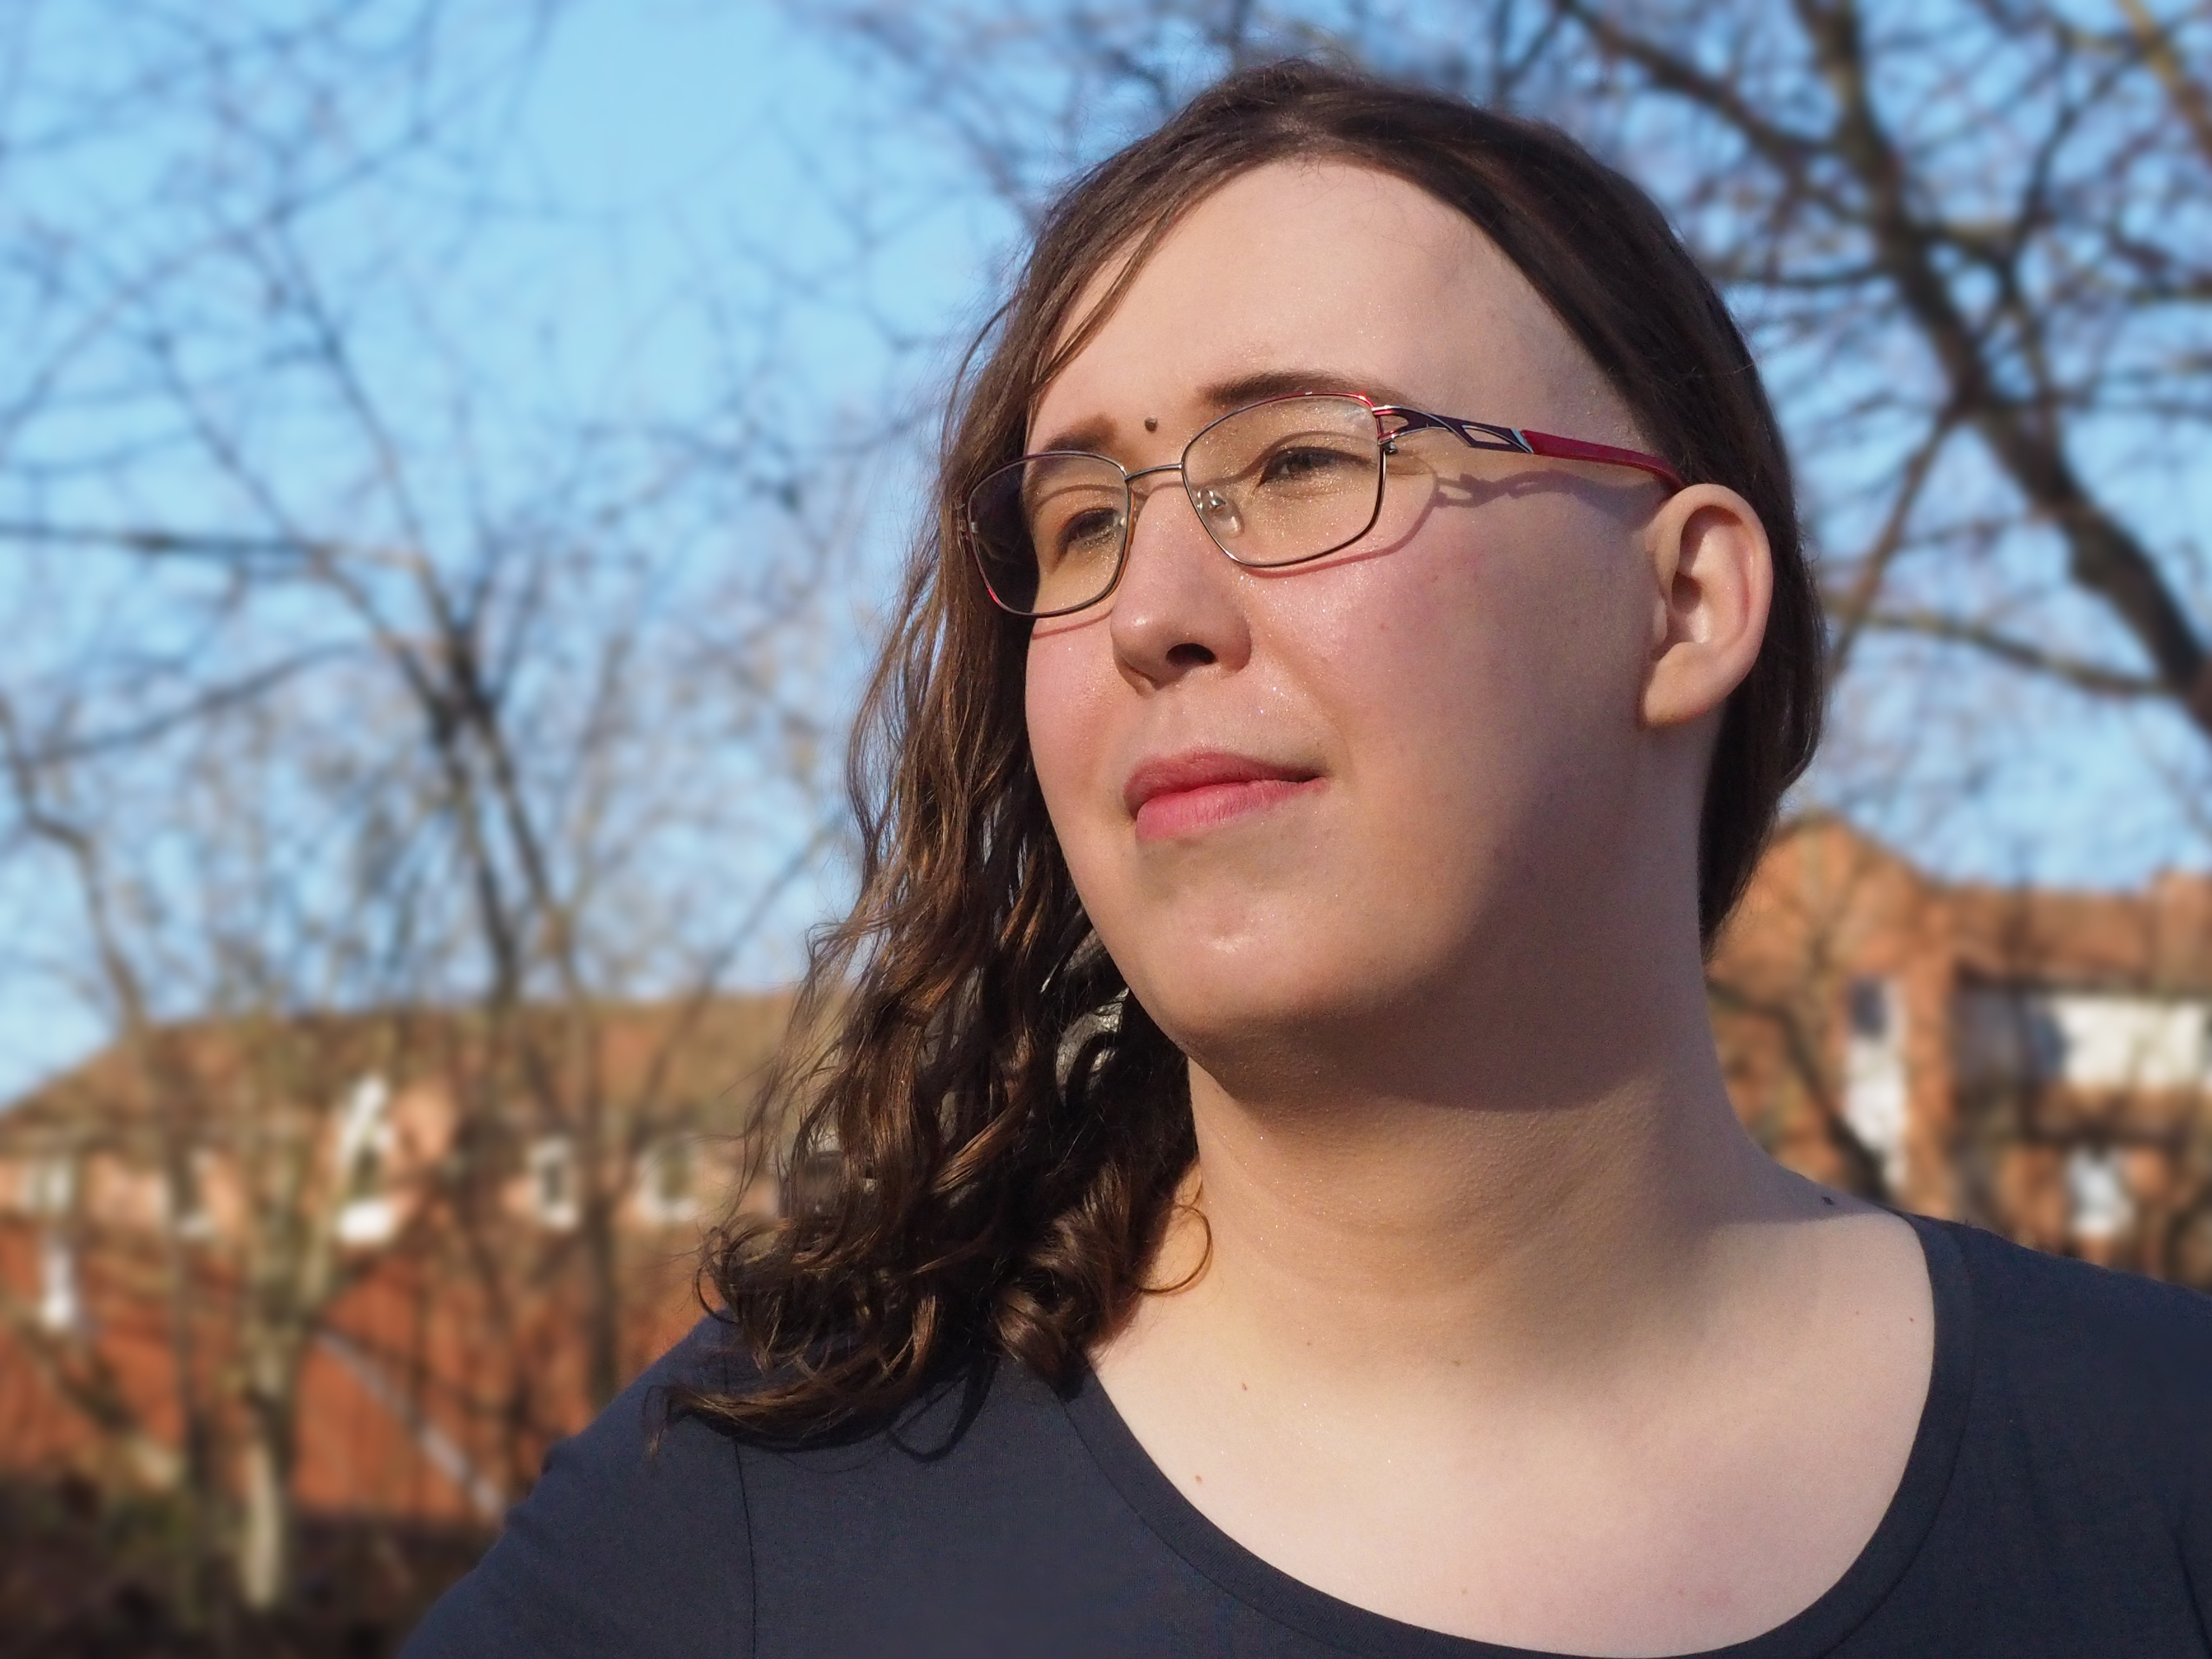
\includegraphics[width=.92\linewidth,trim=200 0 100 0,clip]{graphics/karolin-varner.jpg}
    \end{column}
  \end{columns}
\end{frame}

\begin{frame}{Wanja Zaeske}
  \begin{columns}[fullwidth,c]
    \begin{column}{.3\linewidth}
      
\includegraphics[width=.92\linewidth]{graphics/wanja-zaeske.png}
    \end{column}
    \begin{column}{.7\linewidth}
      \begin{itemize}
        \item Researcher \& Software-Entwickler
        \item 4 Jahre Forschung im Deutsches Zentrum für Luft- und Raumfahrt (DLR)
        \item Schwerpunkt: moderne Softwaretechnologien in die Avionik bringen
        \item Mitgründer von Rosenpass e.V.
      \end{itemize}
    \end{column}%
  \end{columns}
\end{frame}

\begin{frame}{Rosenpass e.V.}
  \begin{columns}[fullwidth,c]
  	\hspace*{.25\LeftSlideIndent}
    \begin{column}{.5\linewidth}
      \begin{itemize}
        \item 2023 gegründet zur Betreuung des gleichnamigen Projekts
        \vfill
        \item Absicherung von WireGuard gegen Attacken durch Quantencomputer mittels protocol-level Hybridisierung
        \item Institution für Translationsforschung in der Kryptografie
        \vfill
        \item Schnittstelle zwischen Forschung, Industrie und Gesellschaft
      \end{itemize}
      \bigskip
      \textbf{\url{rosenpass.eu}}
    \end{column}%
    \begin{column}{.5\linewidth}
%      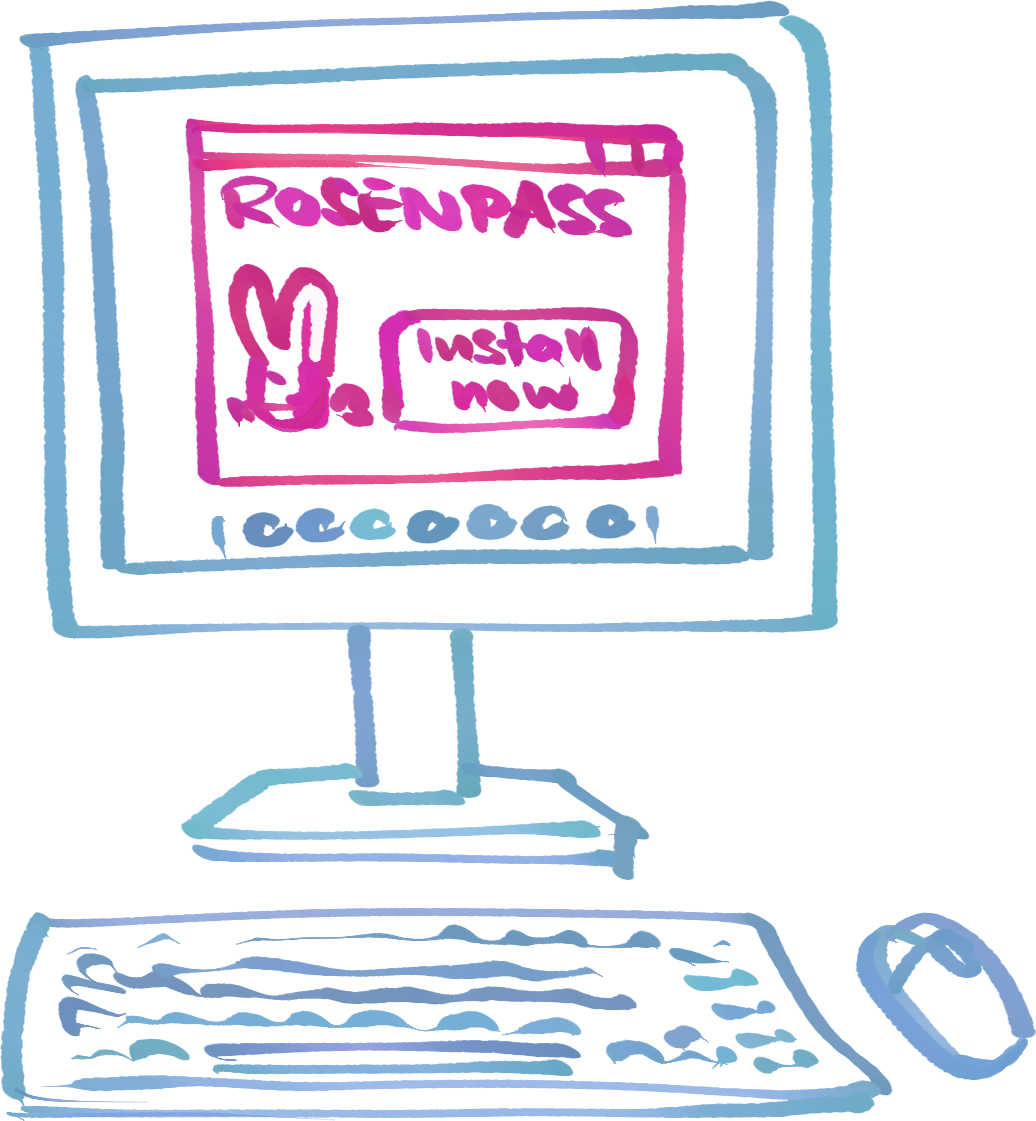
\includegraphics[ width=.92\linewidth]{graphics/Illu-install.png}
		\makebox[\linewidth][c]{\includegraphics[width=1.3\linewidth,page=18]{hpke-slide-designs}\hskip1.5em}
    \end{column}%
  \end{columns}
\end{frame}

\interlude[0]{Safety \& Security \\ \Large \hrule \vspace{1.2em} Kulturelle Aspekte}
\section{Safety \& Security}

\begin{frame}[T]{Safety \& Security in Computersystemen}
% GOAL Beide Begriffe einführen
\small
	% TODO Grafik einfügen
  \begin{columns}[t,fullwidth]
   \hfill
    \begin{column}{.45\linewidth}
      \begin{block}{Safety}
      \begin{itemize}
        \item Schutz von Lebewesen
      % \begin{itemize}
      % \end{itemize}

      \end{itemize}
      \end{block}
    \end{column}
    \hfill
    \begin{column}{.45\linewidth}
      \begin{block}{Security}
      \begin{itemize}
        \item Schutz von Informationen
        \begin{itemize}
          \item Information vor Dritten geheimhalten
          \item Information vor Manipulation durch Dritte schützen
        \end{itemize}
      \end{itemize}
      \end{block}
    \end{column}
    \hfill
  \end{columns}
\end{frame}

\begin{frame}[T]{Problemstellungen \& Rahmenbedingungen}
% GOAL Verfahren sind beim ersten Hinblick inkompatibel, Klar machen, dass beide Begriff verschieden sind und verschiedene Vorgehen erfordern
% TODO Grafik aus Poster einfügen? Problem: Graifk misch Problem, Kultur und Dialog. Grafik ist english.
% Tabelle anstatt grafik
\small
  \begin{columns}[t,fullwidth]
   \hfill
	% TODO make table
    \begin{column}{.45\linewidth}
      \begin{block}{Safety}
      \begin{itemize}
        \item Fehler: Zufällig
        \item Im Fehlerfall: Weiterbetrieb ermöglichen!
        \item Stabile Zieldefinition:\\Physik bleibt gleich
        \item Abgehangene Software $\rightarrow$ Stabil!
        \item Normierte Validierungsprozesse
      \end{itemize}
      \end{block}
    \end{column}
    \hfill
    \begin{column}{.45\linewidth}
      \begin{block}{Security}
      \begin{itemize}
        \item Fehler: Gezielt durch Angreifer
        \item Im Fehlerfall: Lieber das System stoppen
        \item Zieldefinition ist in Bewegung:\\Angreifer lernen dazu
        \item Abgehangene Software $\rightarrow$ Unsicher?
        \item Dynamische Validierungsprozesse
      \end{itemize}
      \end{block}
    \end{column}
    \hfill
  \end{columns}
\end{frame}


\begingroup
\ExplSyntaxOn
\definecolor{green1}{RGB}{48, 175, 155}
\definecolor{green2}{RGB}{130, 221, 207}
\colorlet{green3}{rosenpass-lightblue}
\newcommand*{\Level}[1]{
	\str_case:nnF {#1} {
		{+}{\cellcolor{green3}+}
		{++}{\cellcolor{green2}+\,+}
		{+++}{\cellcolor{green1}+\,+\,+}
		{-}{\cellcolor{red!10}}
	}
	{#1}
}
\ExplSyntaxOff

\begin{frame}[T]{Vertrauen schaffen: Akzeptanzkriterien}
  % GOAL erklären, wie man in Safety/Security Konfidenz erzeugt, einen guten Job gemacht zu haben
%  \begin{table}[]
    \begin{tabular}{l|cc|cc}
      \multirow{2}{*}{\bfseries Kriterium}
        & \multicolumn{2}{c|}{\bfseries Safety}
        & \multicolumn{2}{c}{\bfseries Security} \\ %TODO transpose
                           & \bfseries Konfidenz & \bfseries Verbreitung & \bfseries Konfidenz & \bfseries Verbreitung \\
    \hline
%     \\% TODO (also eigentlich Hinweis) Wanja: Hier ist eine Leerzeile die keine zweite/dritte Spalte hat, daher wird die vertikale linie nicht durchgezogen, aber vertikale linien sind eh doof
	% alternativ &&\\
    Praktische Tests          & \Level{+++}    & \Level{+++}     & \Level{+}           & \Level{++}       \\
    Proven-in-use             & \Level{++}     & \Level{+}       & \Level{-}           & \Level{+}        \\
    Mathematische Beweise     & \Level{+++}    & \Level{-}       & \Level{+++}         & \Level{++}       \\
    Externe Audits            & \Level{++}     & \Level{+++}     & \Level{+++}         & \Level{+++}      \\
    \end{tabular}
      \textbf{Verbreitung} Häufigkeit als tragendes Argument im Assurance-Case\\
      \textbf{Konfidenz} Vertrauen in das Kriterium


  % \begin{itemize}
  %   \item Safety
  %   \begin{itemize}
  %     \item Goldstandard: Requirements-getriebenes Testen % üblich
  %     \item Alternative: "Proven in use" % unüblich
  %     \item Alternative: Formale Verifikation % selten
  %   \end{itemize}

  %   \item Security
  %   \begin{itemize}
  %     \item "Proven in use" reicht nicht, aber neuen Verfahren wird dennoch misstraut
  %     \item Testen unzureichend, aufgrund gezielter Angriffe
  %     \item Formale Verifikation ist der Goldweg
  %   \end{itemize}
  % \end{itemize}

\end{frame}
\endgroup

\begin{frame}[T]{Ingenieurskulturen}
  % GOAL Es gibt Unterschiede, die Begründet sind. Wenn Safety und Security verbunden werden sollen, müssen beide Gründe verstanden werden.
	\begin{columns}[t,fullwidth]
		\hfill
		\begin{column}{.45\linewidth}
			\begin{block}{Safety $\Longrightarrow$ Konservativ}
				\begin{itemize}
				\item Menschen Sterben bei Versagen
				\item Probleme sind Verstanden und Stabil
				\end{itemize}
			\end{block}
		\end{column}
		\begin{column}{.45\linewidth}
			\begin{block}{Security $\Longrightarrow$ Progressive}
				\begin{itemize}
				\item Versagen erzeugt eher finanziellen Schaden
				\item Problemtypen sind dynamisch und ändern sich dauernd
				\end{itemize}
			\end{block}
		\end{column}
		\hfill
	\end{columns}

	% TODO marei center this block?
    \begin{block}{Security + Safety $\Longleftrightarrow$ Konservativ $\lightning$ Progressiv}
	    \begin{itemize}
	      \item Menschen sterben bei Versagen
	      \item Probleme sind dynamisch, Zielsetzung in Bewegung
	    \end{itemize}
  	\end{block}
\end{frame}

\begin{frame}[T]{Safety + Security: Checkliste}
  % GOAL Klar machen, dass beide Domänen nicht unversöhnbar sind
  \begin{enumerate}
	% TODO add checkmarks checkboxes für mehr Checklisten Vibe
	% TODO smallcaps
	% TODO checkbox right aligend
    \item Hohe Zuverlässigkeit
    \item Klarheit über Systemziele
    \item Umfassende Validierung
	\item Unabhängiges Review
    \item Analyse von Softwaresystemen in reeller Hardware
    \item Redundante Systeme
    \item \textbf{Kryptoagilität}
  \end{enumerate}
\end{frame}

% TODO klar benennen, dass wir uns jetzt ein Fallbeispiel Anschauen

\begin{frame}{Die Vier Domänen der Sicherheit sind…}
  % GOAL Orientierung, wo wie gerade hinschauen für das Fallbeispiel
  \Large
  \begin{columns}[c]
    \begin{column}{.5\linewidth}
      \textbf{Luftfahrt}
    \end{column}
    \begin{column}{.5\linewidth}
      Automobile
    \end{column}
  \end{columns}
  \vfill
  \begin{columns}[c]
    \begin{column}{.5\linewidth}
      Medizintechnik
    \end{column}
    \begin{column}{.5\linewidth}
      Automatisierung
    \end{column}
  \end{columns}
\end{frame}

\interlude[1]{Kryptografie in der Avionik}

\begin{frame}[c]{Sichere Kryptografie in der Avionik}
  % TODO: Screenshot von Economy Class cryptography Paper, und von LDACS paper
  % TODO: Both papers in two-column?
  % GOAL Aufzeigen, das (gute) Cryptography in Avionik fehlt
  \vspace{4em}
  \footnotesize
  (Gähnende Leere)
\end{frame}

\begin{frame}[c]{Zum erschrecken aller…}
  % GOAL Aufzeigen, dass auch fortschrittliche Planung durch Mangelnde Kryptoagilität zum scheitern verurteilt ist (LDACS Paper)
  \begin{columns}[fullwidth,c]
    \begin{column}{.5\linewidth}
      \begin{itemize}

        \footnotesize
        …wird in der Luftfahrt heutzutage keine sichere Kryptografie eingesetzt. 

        \vspace{1em}
        Der eine Ernstzunehmende Vorschlag den wir gefunden hatten -- ein System zum kryptografischen absichern von LDACS --
        setzte auf post-quanten chiffren (SIKE), gegen die ein Jahr später Angriffe gefunden wurden.

        % TODO: Insert REFERENCE
      \end{itemize}
    \end{column}%
    \begin{column}{.5\linewidth}
      % GOAL Digital Drahtlos Kommunikation seit 45 jahren
      % GOAL Erste ernste zunehmende Kryptographie in 2007 eingeführt, aber quasi keine Verbreitung
      % GOAL 2021 dann der erste Vorschlag, für einen hybridig post-quaten sicheren Datalink...
      % GOAL ... aber noch vor dem Rollout und nach nur einem Jahr ist die chiffre gebrochen :(
      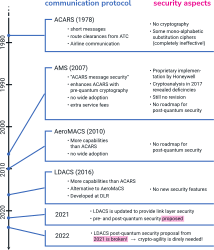
\includegraphics[width=.92\linewidth]{graphics/history of cryptography in avionics}
    \end{column}
  \end{columns}
\end{frame}


\begin{frame}[c]{Kryptographisches Rahmenwerk}
  % TODO check graphics from slides from HACMAS
  % TODO größerere Graphic, in die mitte
  \begin{columns}[fullwidth,c]
    \begin{column}{.65\linewidth}
      \begin{itemize}
        \item HPKE als Schema

        \item Festes Interface
        \begin{itemize}
          \item Seal: Nachricht verschlüsseln (und signieren)
          \item Open: Nachricht entschlüsseln (und prüfen)
        \end{itemize}

        \item Modularität der Primitive
        \begin{itemize}
          \item KEM: Key Encapsulation Funktion\\Eigener Privater Schlüssel, Öffentlicher Schlüssel Addressat $\rightarrow$ Sym. Schlüssel
          \item KDF: Key Derivation Function\\Schlüsselmaterial, Entropie $\rightarrow$ Schlüssel
          \item AEAD: Authenticated Encryption with Associated Data\\
            Symetrische Chiffre mit Authentisierung\\
            Klartext, Sym. Schlüssel $\rightarrow$ Cyphertext\\
            Cyphertext, Sym. Schlüssel $\rightarrow$ Klartext. Authentisiert?
        \end{itemize}

        % TODO placement and size of graphics
      \end{itemize}
    \end{column}%
    \begin{column}{.35\linewidth}
      
        \includegraphics[width=0.8\linewidth]{graphics/hpke}
        % TODO explain every detail of this Graphic
    \end{column}
  \end{columns}
\end{frame}


\begin{frame}[c]{Bedarfsgerechte Security}
  \begin{columns}[fullwidth,c]
    \begin{column}{.35\linewidth}
      \begin{itemize}
        \item Pre oder Post-Quantum?
        \item Mehr oder weniger Speicherbedarf?
        \item Schenelle or langsame Berechnung?
        \item Post-quantum Authentisierung? 
      \end{itemize}
    \end{column}%
    \begin{column}{.65\linewidth}
      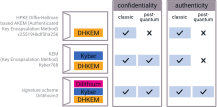
\includegraphics[width=\linewidth]{graphics/hpke variants}
    \end{column}
  \end{columns}
\end{frame}


\begin{frame}[c]{Integration in die Avionik}
  \begin{columns}[fullwidth,c]
    \begin{column}{.4\linewidth}
      \begin{itemize}
        \item Bündelung der Kyrypto-Implementierung
        \item Modul der Avionik: Partition\footnote{Partitionen sind voneinander isoliert, und dürfen daher in der Zulassung separat betrachtet werden}
        \item Einfacher Austausch der Krypto-Partition
      \end{itemize}
      \vspace{8.5em} % TODO This is a hack, maybe marei can fix it?
    \end{column}%
    \begin{column}{.6\linewidth}
      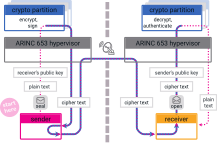
\includegraphics[width=\linewidth]{graphics/crypto partition}
    \end{column}
  \end{columns}
\end{frame}

% GOAL Aufzeigen, dass und wie Modularität der Schlüssel für Kryptoagilität in der Safety ist
% GOAL Aufzeigen, dass Integration einfach möglich, und zulassungsfreundlich gemacht werden kann


% TODO eine folie über Benchmarks?


% \begin{frame}[c]{Ansätze für Verbesserung in beiden Bereichen}
%   % GOAL ist mir unklar
%   % TODO wucke refine 

%   Verifikationstechniken
%   \vspace{0.5em}

%   {\footnotesize Zertifizierung <-> Sicherheitsbeweise}
%   \vspace{1.5em}
%   % Formaler Beweis kann Teil der Evidence für Zertifizierung sein
%   % Annahmen und Anforderungen müssen in den Zertifizierungsdokumenten festgehalten werden
%   % Evidence = Belege, warum Annahmen wahr sind oder Anforderungen erfüllt sind
%   % Unabhängigkeit zwischen Implementierer und Verifizierer
%   % 
%   % - Wanja
%   %
%   % Agreed; geht mir eher darum die generelle Vorgehensweise zu beschreiben als formell korrekt jede Möglichkeit durchzugehen.
%   % Ist beweisführung in der Avionik denn üblich?
%   % 
%   % – Karolin

%   Kompartmentalisierung
%   \vspace{0.5em}

%   {\footnotesize Partitionierung <-> Brokerarchitekturen}
%   \vspace{1.5em}
%   % Aufteilung erleichtert sukzessive Absicherung einzelner Komponent
%   % Gleichzeitig: Faultcontainment
%   % Modularisierung macht updates einfacher, da klare interfaces zwischen Modulen

%   % Diagram Idee: Konfidenzarchitektur
%   %
%   % 1. Identifiziere mögliche Fehlerursachen
%   % 2. Ist ein Fehler relevant?
%   %   - Falls Nein, warum nicht? Evidence!
%   % 3. Welche Effekte hat der Fehler?
%   % 4. Wie kann der Fehler verhindert/eingedämmt/mitigiert werden?
%   % 5. Wie kann der Fehler erkannt werden?
%   % 6. Validiere Annahmen von 3. - 5.
%   % 7. Review durch unabhängigen Assesor
%   %
%   % -- wucke13
%   %
%   % Passt das denn in das Gegenüberstellungsscheme? Also wie bringen wir den Vergleich Avionik vs Crypto rein.
%   %
%   % -- karolin

%   => Kryptoagilität
% \end{frame}

\input{00400_agilität_als_prozess}
\input{00500_kryptoaglität_definition}


\end{document}
